% ==========================================
% Thesis Report - Initial Situation ( brods1 )
% ==========================================

\section{Initial System Setup}

\section{CAVE Hardware}
\label{sec:cave_hardware}
The \gls{cpvr} research group of the \gls{bfhti} runs a \gls{cave}. A \gls{cave} is an immersive virtual reality environment. Currently, there are three screens arranged in an open cube geometry where each screen measures about 2x2 meters. Figure \ref{fig:cave} shows the mentioned \gls{cave}.
\begin{figure}[H]
	\centering
	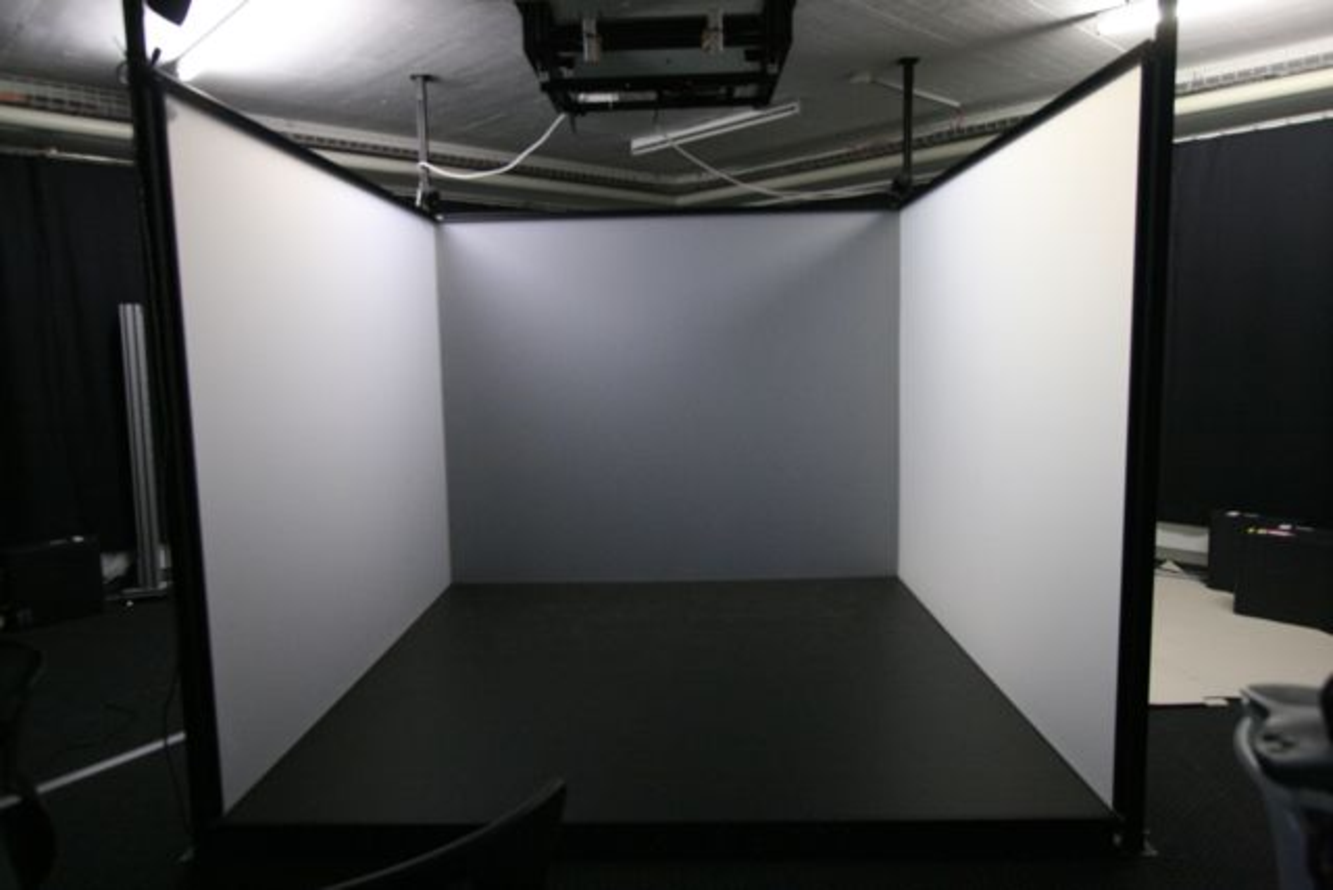
\includegraphics[width=0.5\textwidth]{../figures/fotos/emptyCave}
	\caption{CAVE BFH-TI}
	\label{fig:cave}
\end{figure}

Two projectors are installed on each side of the cube pointing to the particular screen via a mirror. In front of the lens of each projector is one polarization filter fixed, one for left circular polarisation and one for right circular polarisation for each projector pair on each side. The projections on the screen have to match exactly in order to get a proper alignment. A projector pair is shown in Figure \ref{fig:projectors}. One such pair is installed on each side.

\begin{figure}[H]
	\centering
	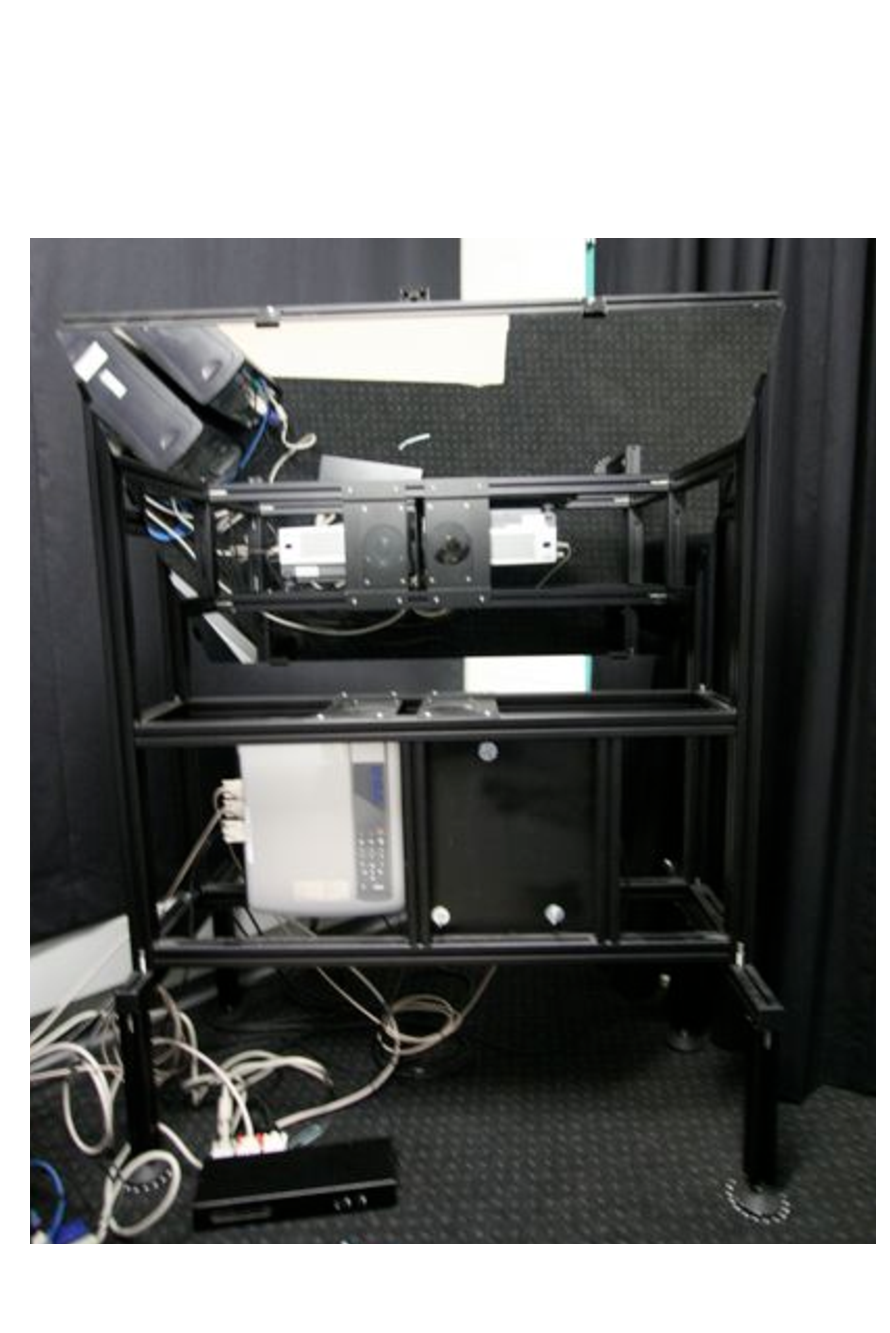
\includegraphics[width=0.3\textwidth]{../figures/fotos/projectors}
	\caption{CAVE projectors}
	\label{fig:projectors}
\end{figure}

There are two additional projectors fixed at the ceiling. They are planned to project to the floor, which is going to increase the immersion of the whole installation as soon as the calibration is done.

The \gls{cave} operates with six render clients and one server. Each client is connected to one of the projectors. The server is responsible to coordinate the different clients. A diagram of this setup is shown in Figure \ref{fig:cave_diagram}.

\begin{figure}[H]
	\centering
	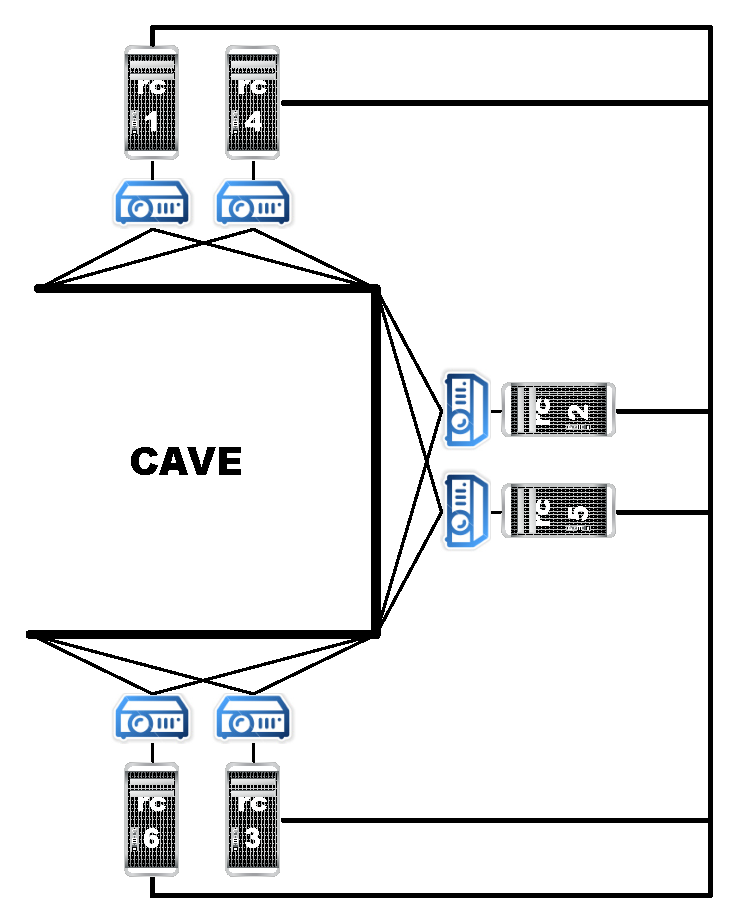
\includegraphics[width=0.6\textwidth]{../figures/6node_architecture}
	\caption{CAVE Hardware Setup}
	\label{fig:cave_diagram}
\end{figure}

For rendering a three dimensional scene in the \gls{cave}, the two clients on each side have to render the same part of the scene so one has the same part of the scene twice on each screen. 
The two projections on each screen have to be rendered with a slightly different position of the camera in order to get a stereoscopic image. The spatial difference has to configured in the software rather physically and should equal the distance between the right and the left eye of the spectator.

To get the three dimensional feeling in the \gls{cave}, one has to wear polarisation glasses (see Figure \ref{fig:glasses}). The effect of these glasses is, that one can only see one image per eye on each wall. This leads to a three dimensional stereoscopic effect.

\begin{figure}[H]
	\centering
	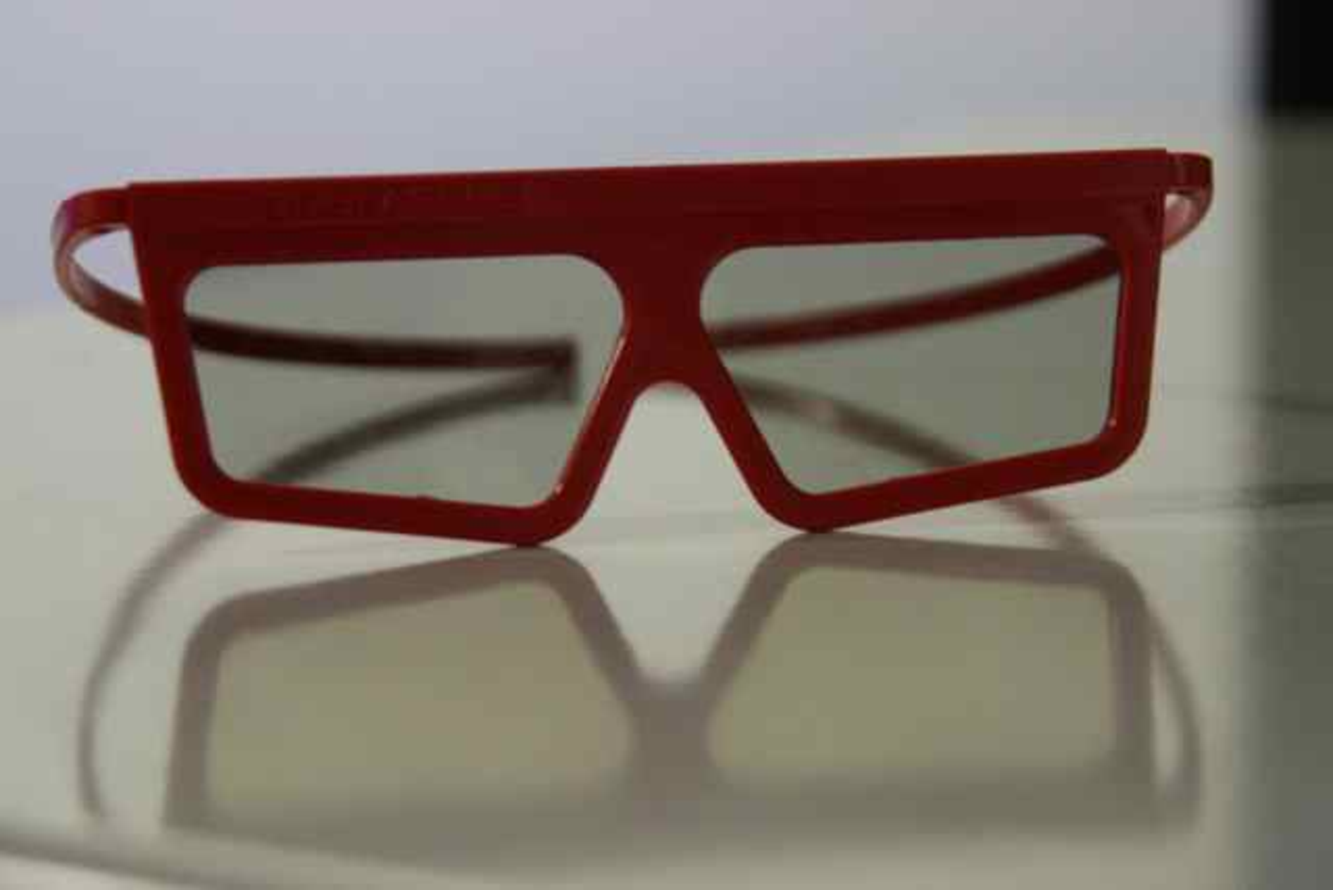
\includegraphics[width=0.4\textwidth]{../figures/fotos/glasses}
	\caption{Polarisation glasses}
	\label{fig:glasses}
\end{figure}

\section{Current CAVE Software Solution}
At the moment, there are two given software architectures in use for the \gls{cave} environment. One is using the Chromium Library for network distributed \glsentrytext{opengl} rendering. For the other one, a distributed VRML/X3D solution is used. The latter uses only minimal network resources, but is limited to VRML/X3D implemented applications.
% explanation of vrml and x3d

\section{Chromium}
One of the currently used frameworks in the \gls{bfhti} \gls{cave} is Chromium\cite{website:chromiumWeb}. Chromium is a flexible framework for scalable real-time rendering on clusters of workstations, derived from the Stanford WireGL project code base. Details concerning the differences between Chromium and Equalizer can be read in the Technical Documentation. We only describe the setup used in the \gls{cave} of the \gls{cpvr} research group.

To avoid further terminology misunderstandings we first want to describe the terms client and server in coherence with the \gls{cave}.

\begin{description}
	\item[client] \hfill\\A client refers to applications which use some servers rendering capabilities.
	\item[server] \hfill\\A server refers to services which do the actual rendering.
\end{description}

Considering this terminology the \gls{cpvr} \gls{cave} consists of seven computers where one of them is the application server and the other six represent the rendering clients. Each of the rendering clients is connected to a projector. There are two projectors for each screen as described in the section above (\nameref{sec:cave_hardware}).

In the setup used by Chromium, the application server takes the role of a client and the rendering clients act as servers. This means there are six servers and one client in the setup.  Chromium leads to a high workload of network traffic.

\section{VRML/X3D}
The other setup used in the \gls{cpvr} \gls{cave} is based on \gls{vrml} and X3D. 
\begin{description}
	\item[VRML\cite{website:VRML}] \hfill\\\gls{vrml} is a standard file format for the representation of 3D vector graphics that may be interactive.
	\item[X3D\cite{website:X3D}] \hfill\\X3D is the ISO standard XML based file format used to represent 3D computer graphics. It is the successor of \gls{vrml}. X3D features extensions to VRML.
\end{description}

This setup is much less network demanding but not less problematic. All applications have to be implemented in \gls{vrml}/X3D. This is a big restriction and allows mostly self proprietary developed applications.

\section{Requirements for the new solution}
In the previous section the two currently running setups were described. Both of them have major disadvantages: Chromium is too network intense and \gls{vrml}/X3D is restricted to a very limited number of applications. Therefore the goal of a new approach was to get a setup that supports distributed rendering without a high network usage and allows to run off-the-rack applications or at least supports a framework that is more common and less restricted that \gls{vrml}/X3D. 
